\section{Problem Description}
In this project we will determine under what conditions it is possible to perform gaze estimation using machine learning.
Gaze estimation is the process of identifying where a person is looking.

To do this we will set up a controlled experiment where test-subjects are looking at 4 points under different conditions.
The 4 points are 4 LED lights mounted in a straight line on a plastic-frame attached to a Genius iSlim 321R web-cam.
See figure \ref{fig:webcamsetup} for a picture of the set-up, and for more information see section \ref{sub:Set-up}.

\begin{figure}[h!]
\centering
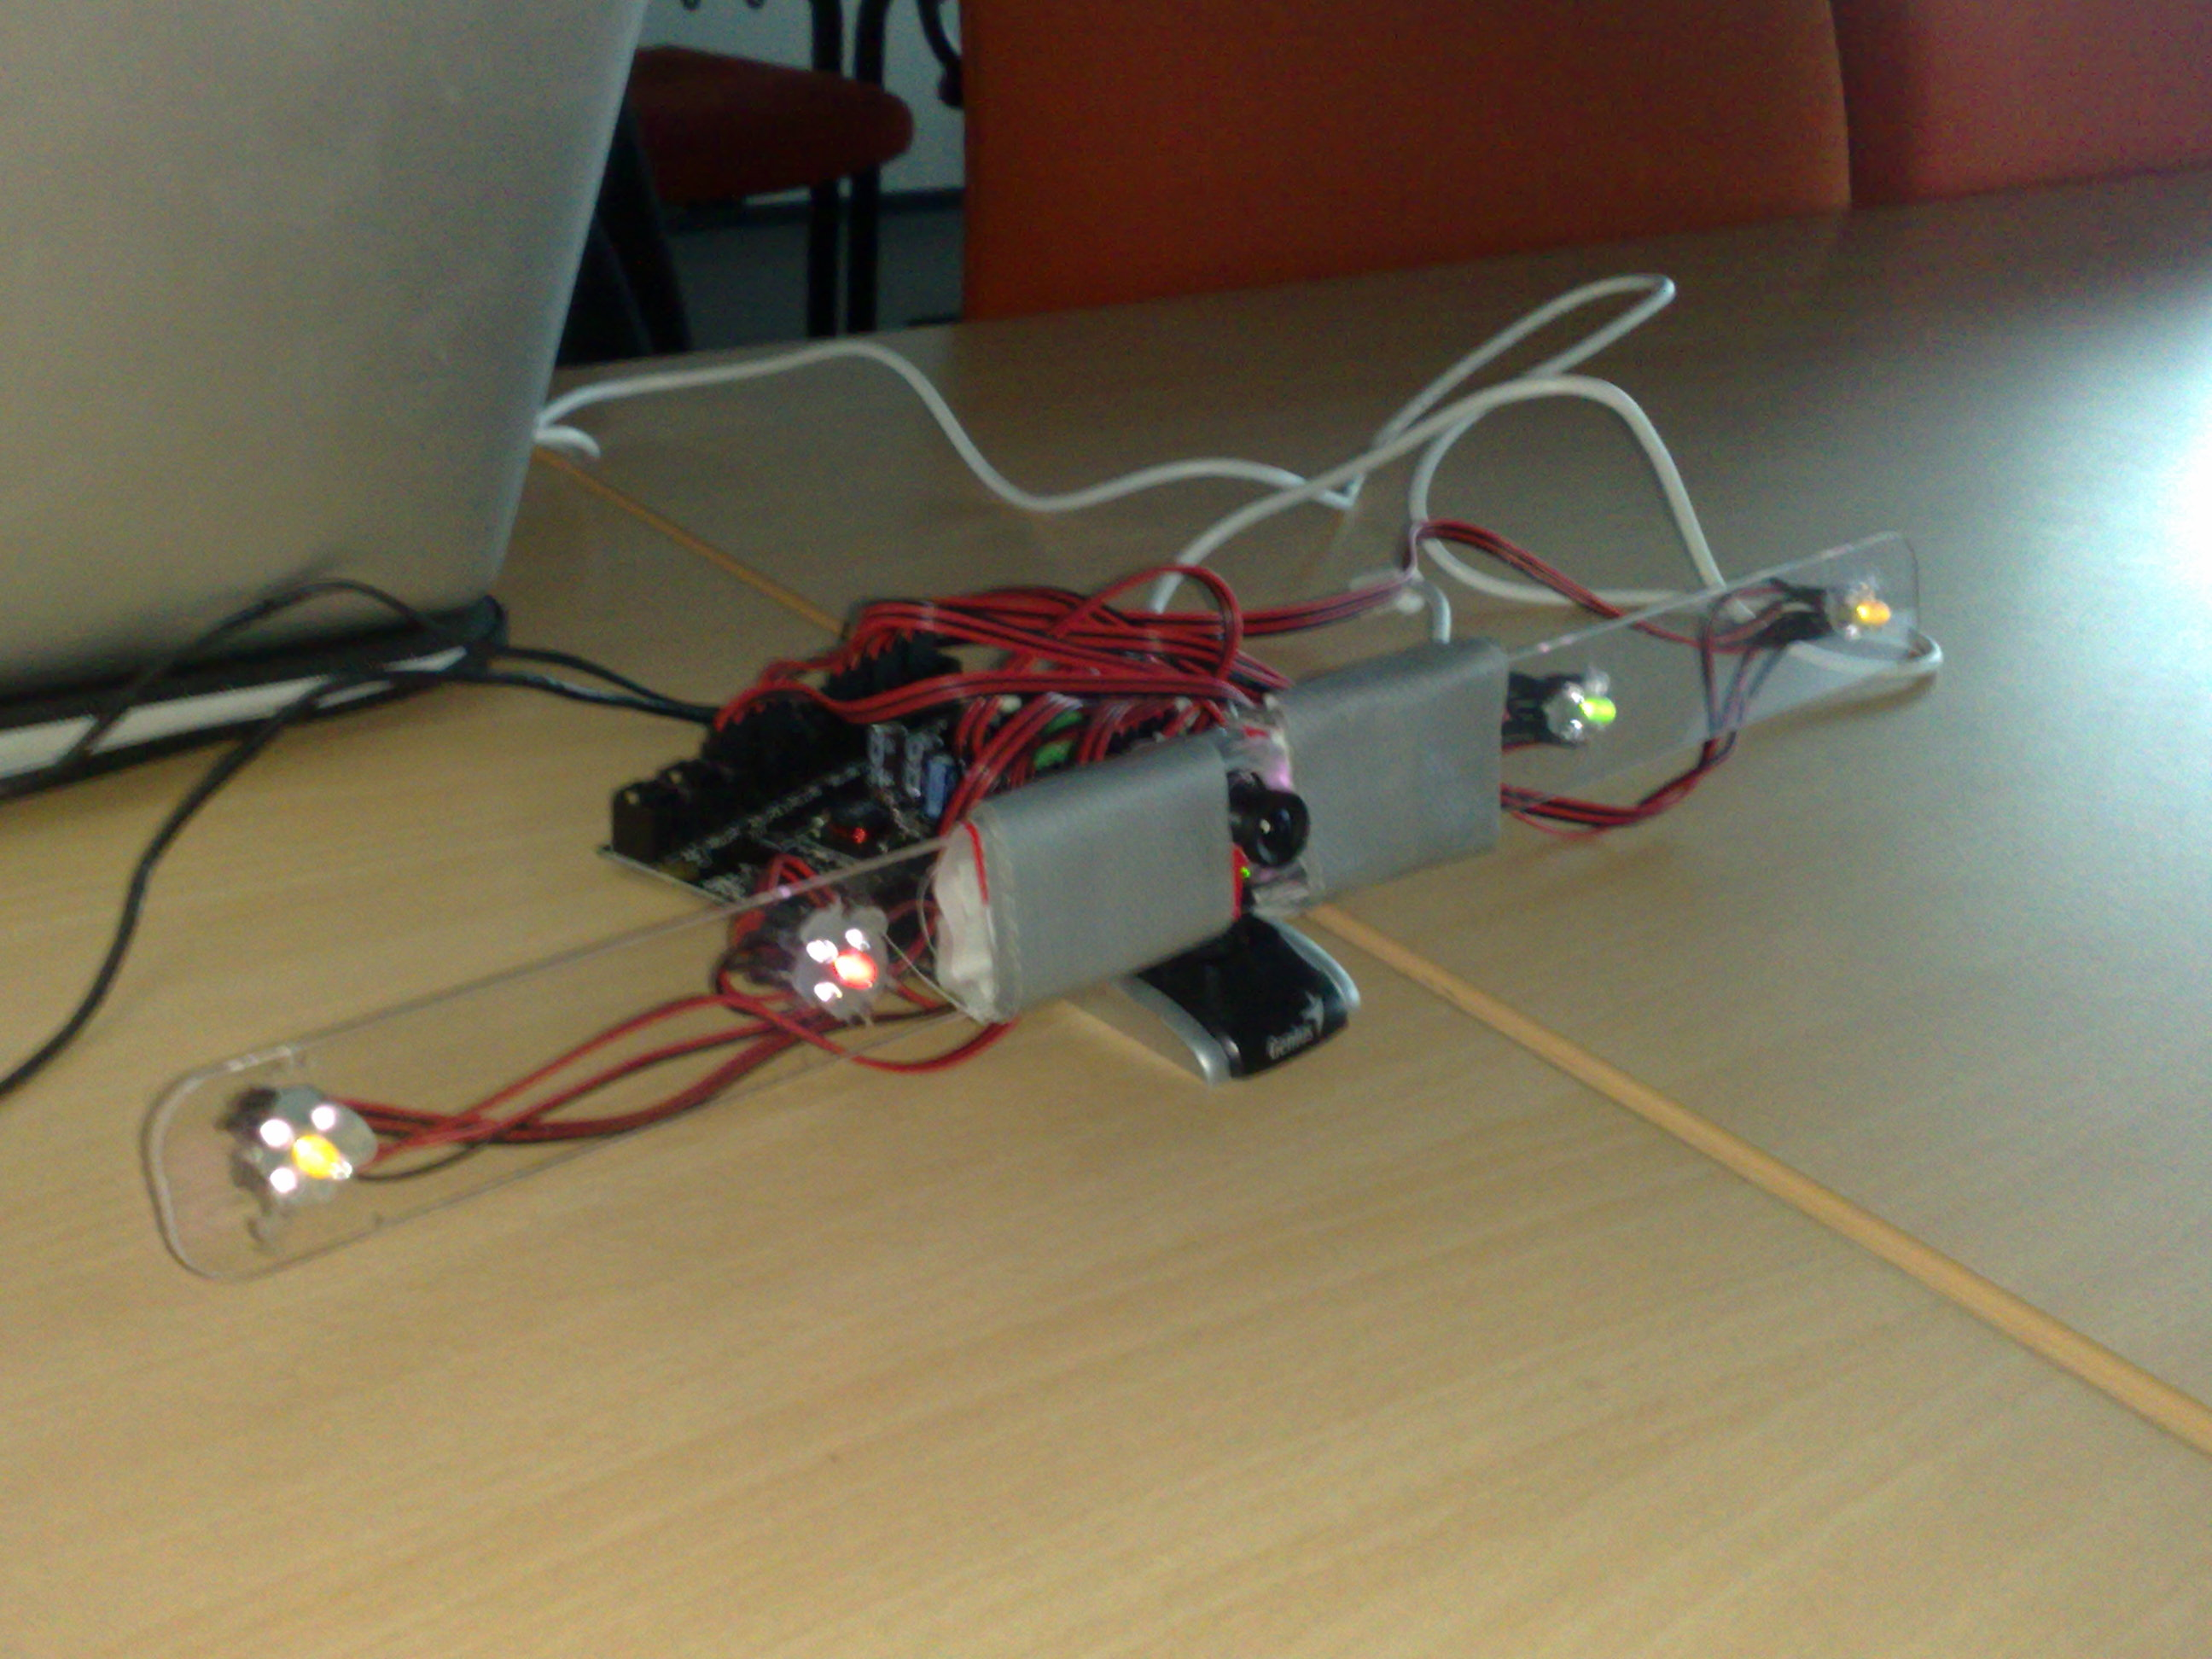
\includegraphics[width=0.8\textwidth]{cameratest}
\caption{Genius iSlim 321R with mounted LED- and infra-red lights.}
\label{fig:webcamsetup}
\end{figure}

We will record videos of the test-subjects looking at the different points under different conditions, and then extract images from the videos.
For more information on the experiment set-up, see section \ref{sub:Experiment}.

The eyes will then be separated from the rest of the image and will be normalized and scaled to a set size.
We will then run Principal Component Analysis, an unsupervised learning algorithm, on the images and analyse in which principal components the different points are separable from each other.
We will also analyse what effect the various conditions have on the outcome. %Kommer vi til det ordentligt?
For more information on Principal Component Analysis, see section \ref{sub:PCA}.

Finally, we will make an algorithm that can determine where a new image of an eye is looking.
We do this using various machine learning algorithms to classify how the different points are best partitioned.

%Gaze estimation is the process of identifying where an eye is looking.
%It has a lot of applications, for example in giving disabled people the ability to type with, and control devices using, their eyes.
%People with Amyotrophic Lateral Sclerosis (ALS) can especially make use of this technology.
%It is also closely related to eye-feature-extraction using image-analysis.
%Eye-feature-extraction can be used to identify eye-features such as corners of the eye, centre of the iris, reflections of light in the eye and so on.
%We will not be using eye-feature-extraction using image-analysis as it is outside the scope of this project.

%Using machine learning for gaze estimation has its issues, as images of faces (or eyes) are high-dimensional data, making learning complex and time-consuming.
%There are a few approaches to reducing this complexity.
%One could reduce the input space by converting the image to grayscale, isolating the eye-pixels from the rest of the image, and scaling the resulting image to a size where learning is feasible.
%One could also reduce the input space by extracting features of the eye such as the positions of the corners of the eye and the centre of the pupil.
%In this project we attempt the first approach.



%When gathering test data there are also many factors to consider.
%Test subjects should be placed similarly in such a way that their eyes are clearly visible to the camera and at a distance where glints in the eyes from infra-red lights are visible.
%The angle of the head and eyes can also impact learning immensely, as they make the eyes look very different compared to a front-facing eye.
%To combat this, one could attempt to rotate the eye, but this may cause other problems.
%Lighting is also very important and should be consistent during testing.

%When processing the initial test data, it can be beneficial to histogram equalize the images to increase the contrast.
%This makes potential lighting issues have less of an impact.